\section{Deployment Aplikasi}

Setelah proses pengembangan selesai dilakukan secara lokal, tahap selanjutnya adalah melakukan \textit{deployment} agar aplikasi dapat diakses oleh pengguna melalui jaringan internet. Dalam penelitian ini, proses \textit{deployment} dilakukan menggunakan platform \textit{Vercel}, yang secara khusus mendukung \textit{framework} \textit{Next.js} dan memungkinkan integrasi otomatis dengan sistem kontrol versi seperti \textit{GitHub}.
\singlespacing{}
Langkah pertama adalah membuka situs \url{https://vercel.com}, kemudian melakukan \textit{login} atau \textit{registrasi} apabila belum memiliki akun. Setelah berhasil masuk, pengguna dapat membuat proyek baru dengan menekan tombol \texttt{New Project}, seperti ditunjukkan pada Gambar~\ref{fig:buat-project}.

\begin{figure}[H]
  \centering
  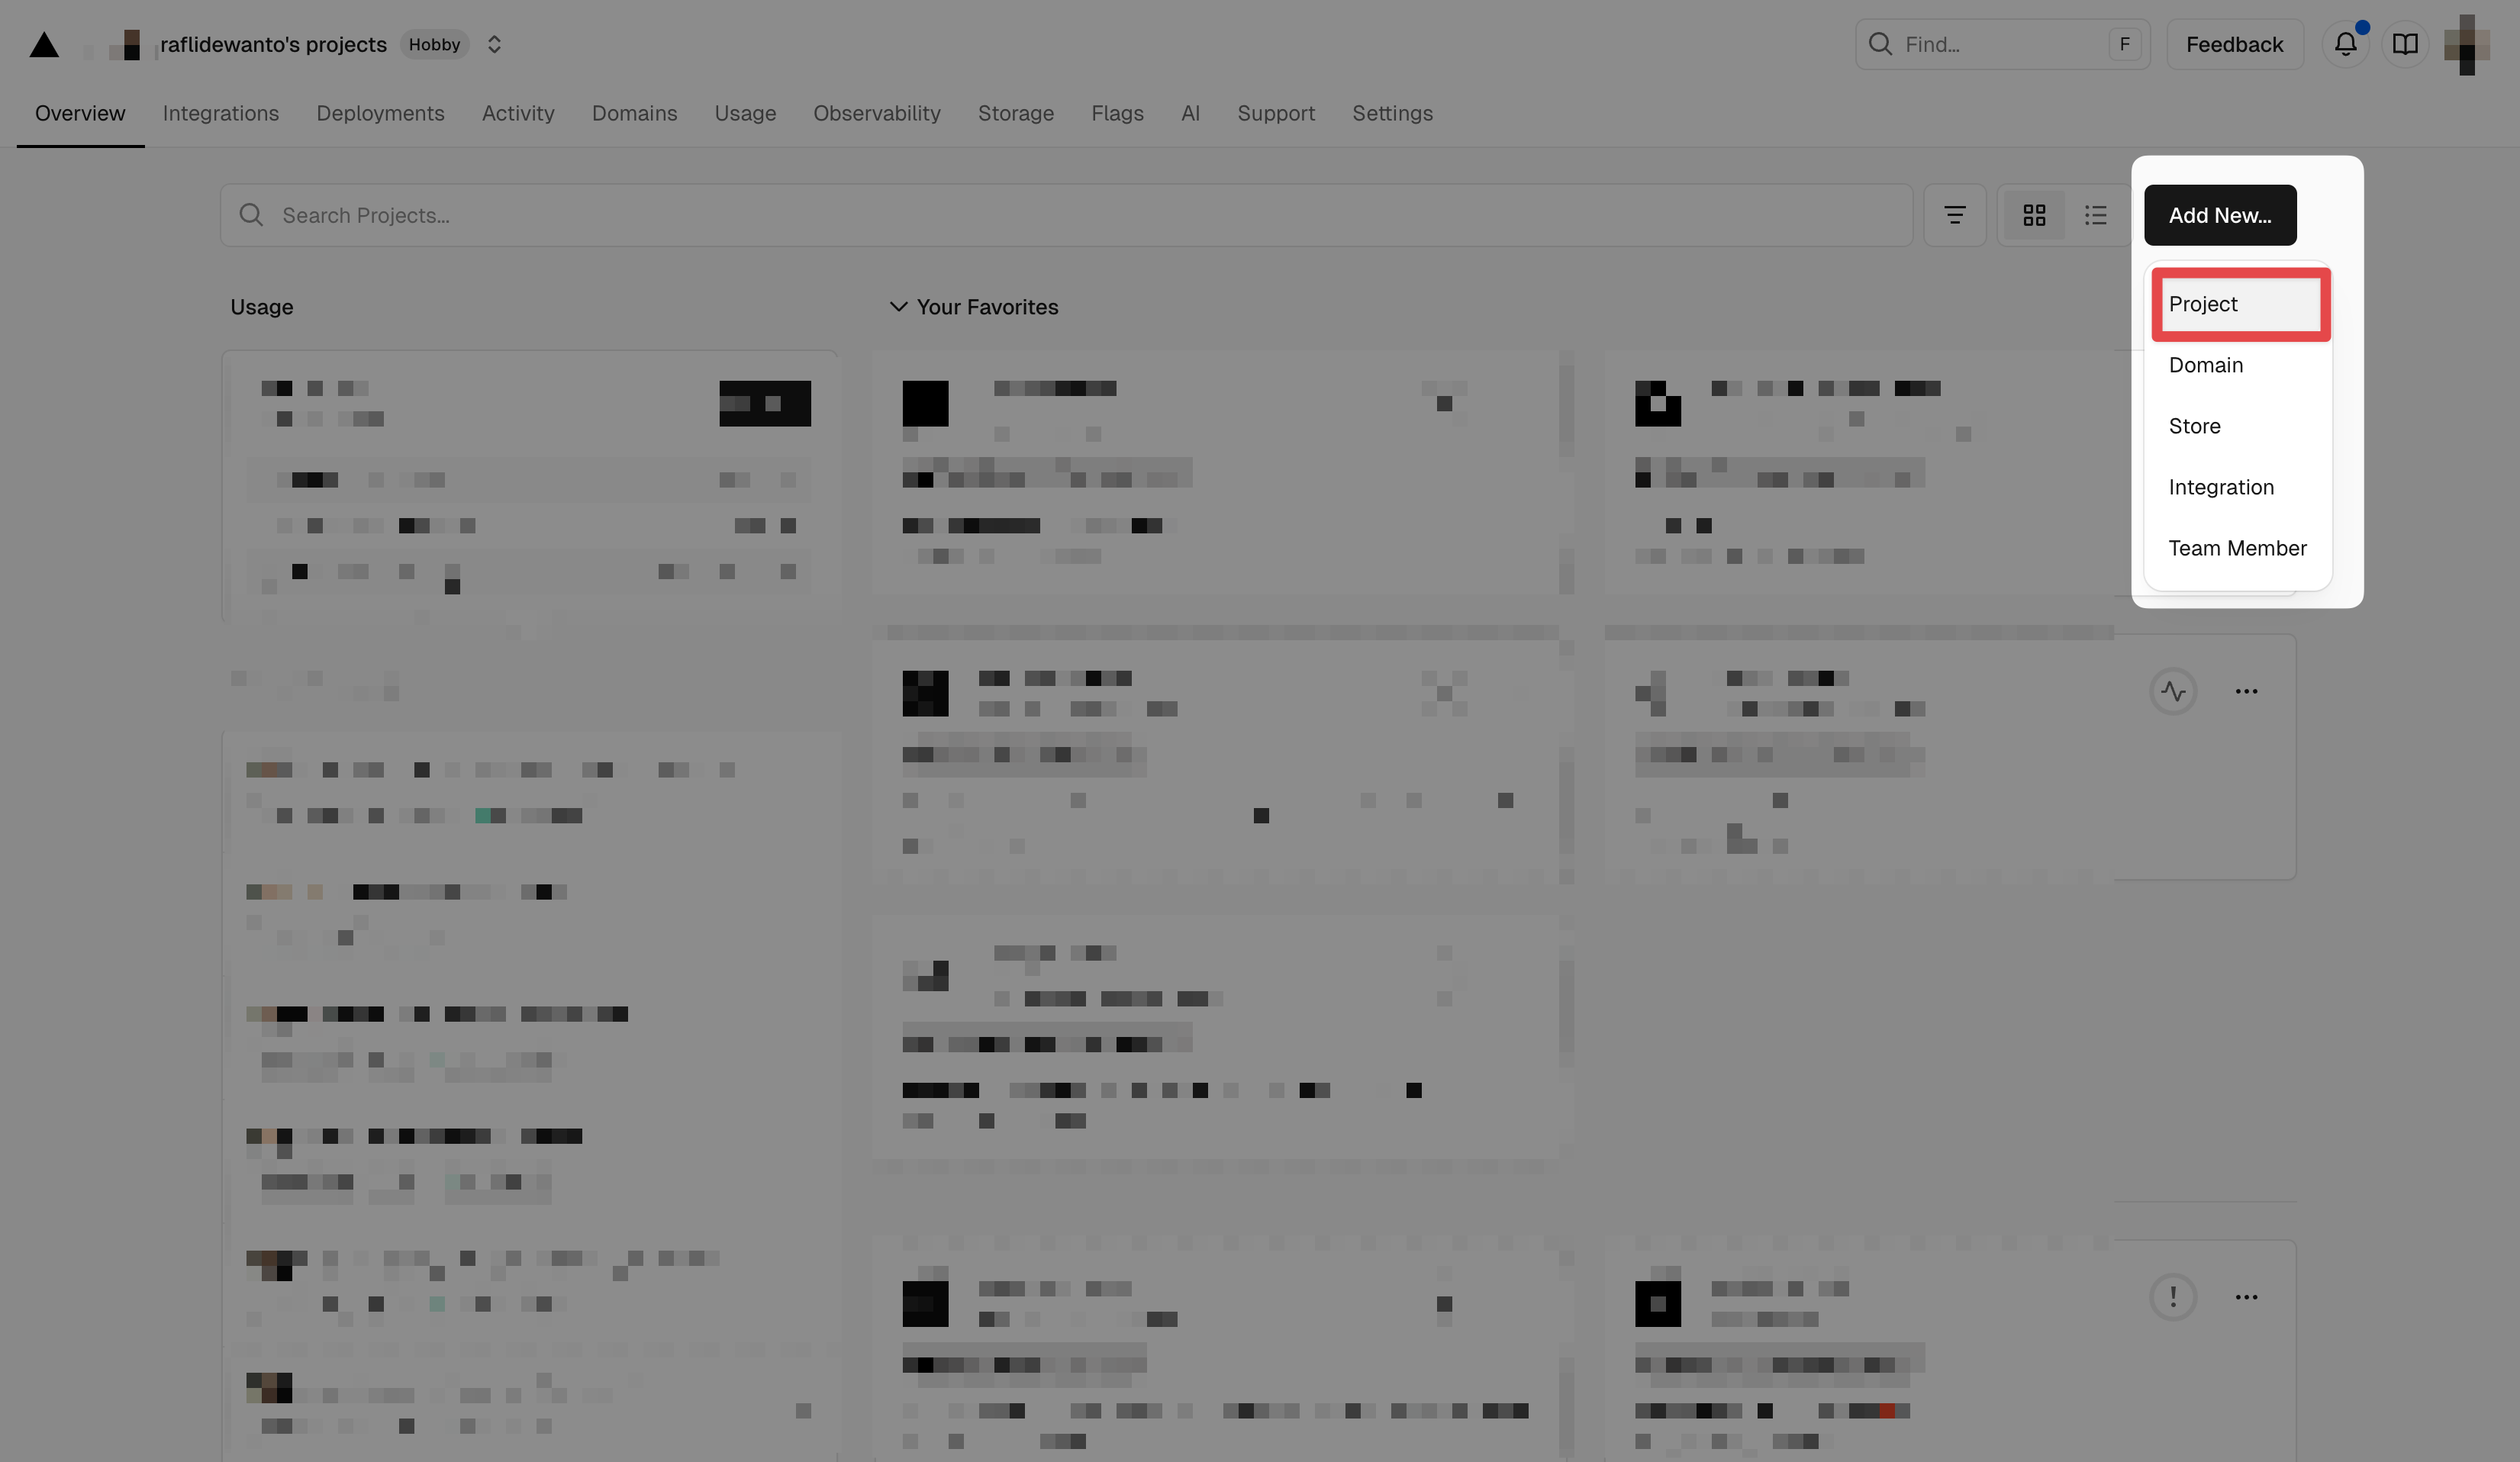
\includegraphics[width=0.85\linewidth]{images/bab-3/deploy-1.png}
  \caption{Membuat proyek baru di Vercel}\label{fig:buat-project}
\end{figure}

Setelah itu, pengguna diminta untuk memilih \textit{repository} yang berisi kode sumber aplikasi. Vercel akan mendeteksi struktur proyek dan framework yang digunakan secara otomatis. Pilih repository yang sesuai, lalu klik tombol \texttt{Import}, seperti diperlihatkan pada Gambar~\ref{fig:pilih-repository}.

\begin{figure}[H]
  \centering
  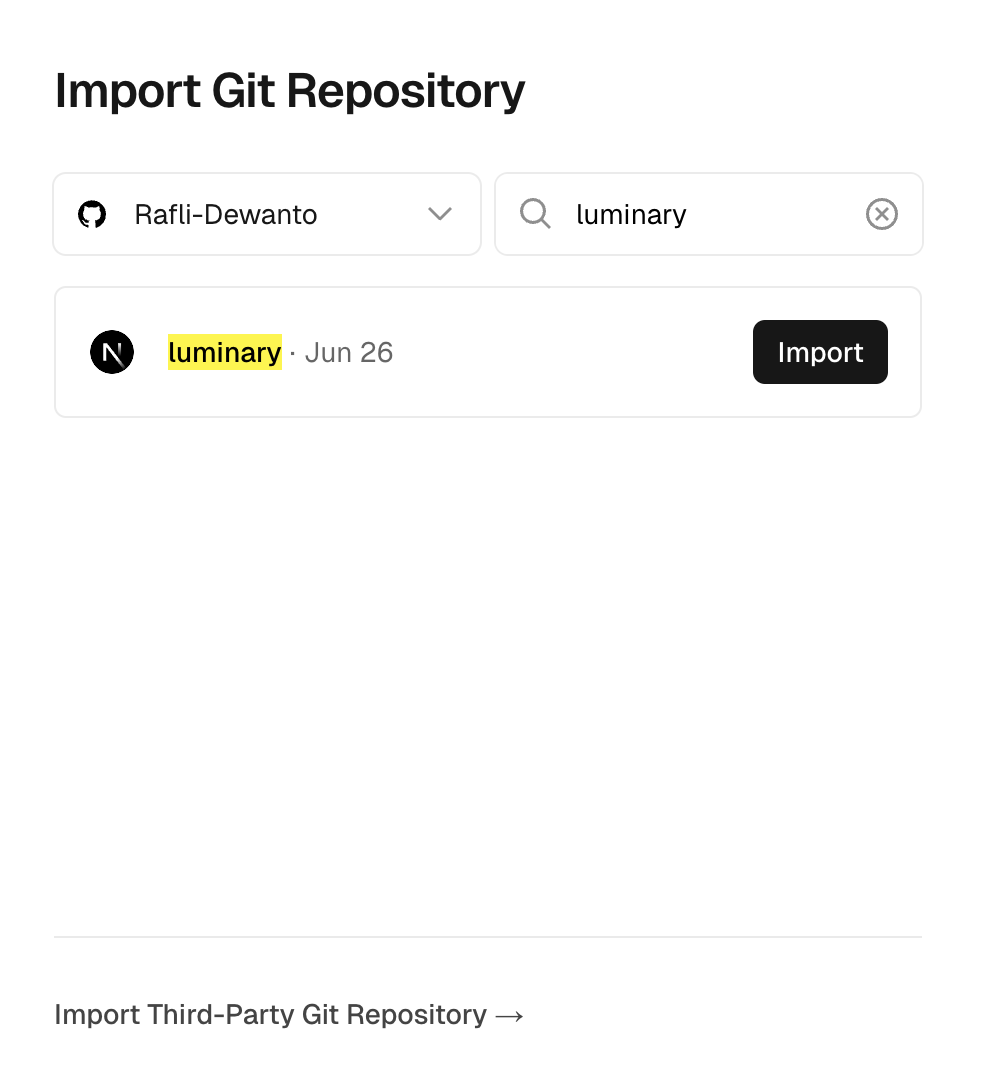
\includegraphics[width=0.85\linewidth]{images/bab-3/deploy-2.png}
  \caption{Mengimpor repository dari GitHub ke Vercel}\label{fig:pilih-repository}
\end{figure}

Langkah berikutnya adalah memasukkan seluruh \textit{Environment Variables} yang diperlukan agar aplikasi dapat berjalan dengan baik. Variabel ini meliputi konfigurasi untuk koneksi ke database PostgreSQL yang dihosting di Neon, token OpenAI API, URL object storage dari Vercel Blob, dan kredensial Redis dari Upstash. Semua variabel harus dimasukkan dengan benar pada tahap ini. Setelah semua siap, klik tombol \texttt{Deploy} seperti terlihat pada Gambar~\ref{fig:deploy-project}.

\begin{figure}[H]
  \centering
  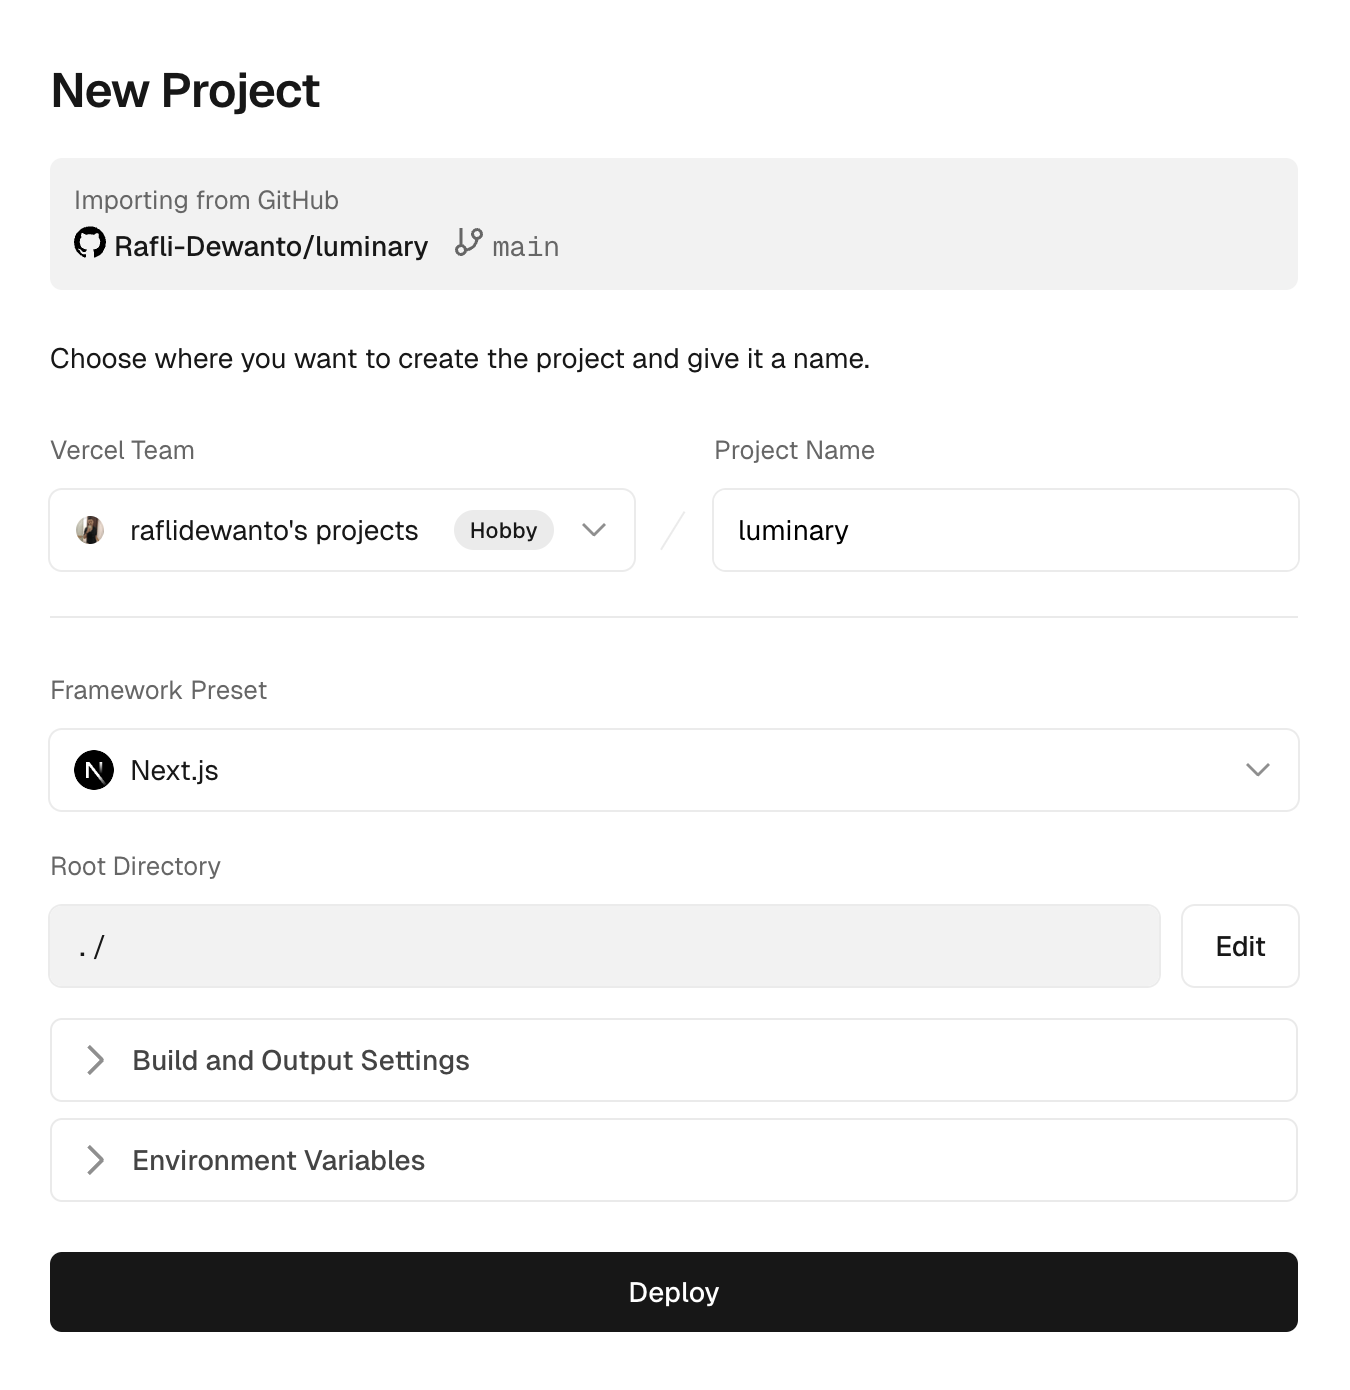
\includegraphics[width=0.85\linewidth]{images/bab-3/deploy-3.png}
  \caption{Menambahkan environment variables dan melakukan deployment}\label{fig:deploy-project}
\end{figure}

Jika semua konfigurasi telah sesuai, proses \textit{deployment} akan berjalan secara otomatis. Setelah proses selesai, Vercel akan menyediakan URL publik untuk aplikasi yang telah berhasil diunggah, seperti diperlihatkan pada Gambar~\ref{fig:finish-deploy}. Dengan demikian, aplikasi dapat langsung diakses oleh pengguna tanpa perlu konfigurasi server tambahan.

\begin{figure}[H]
  \centering
  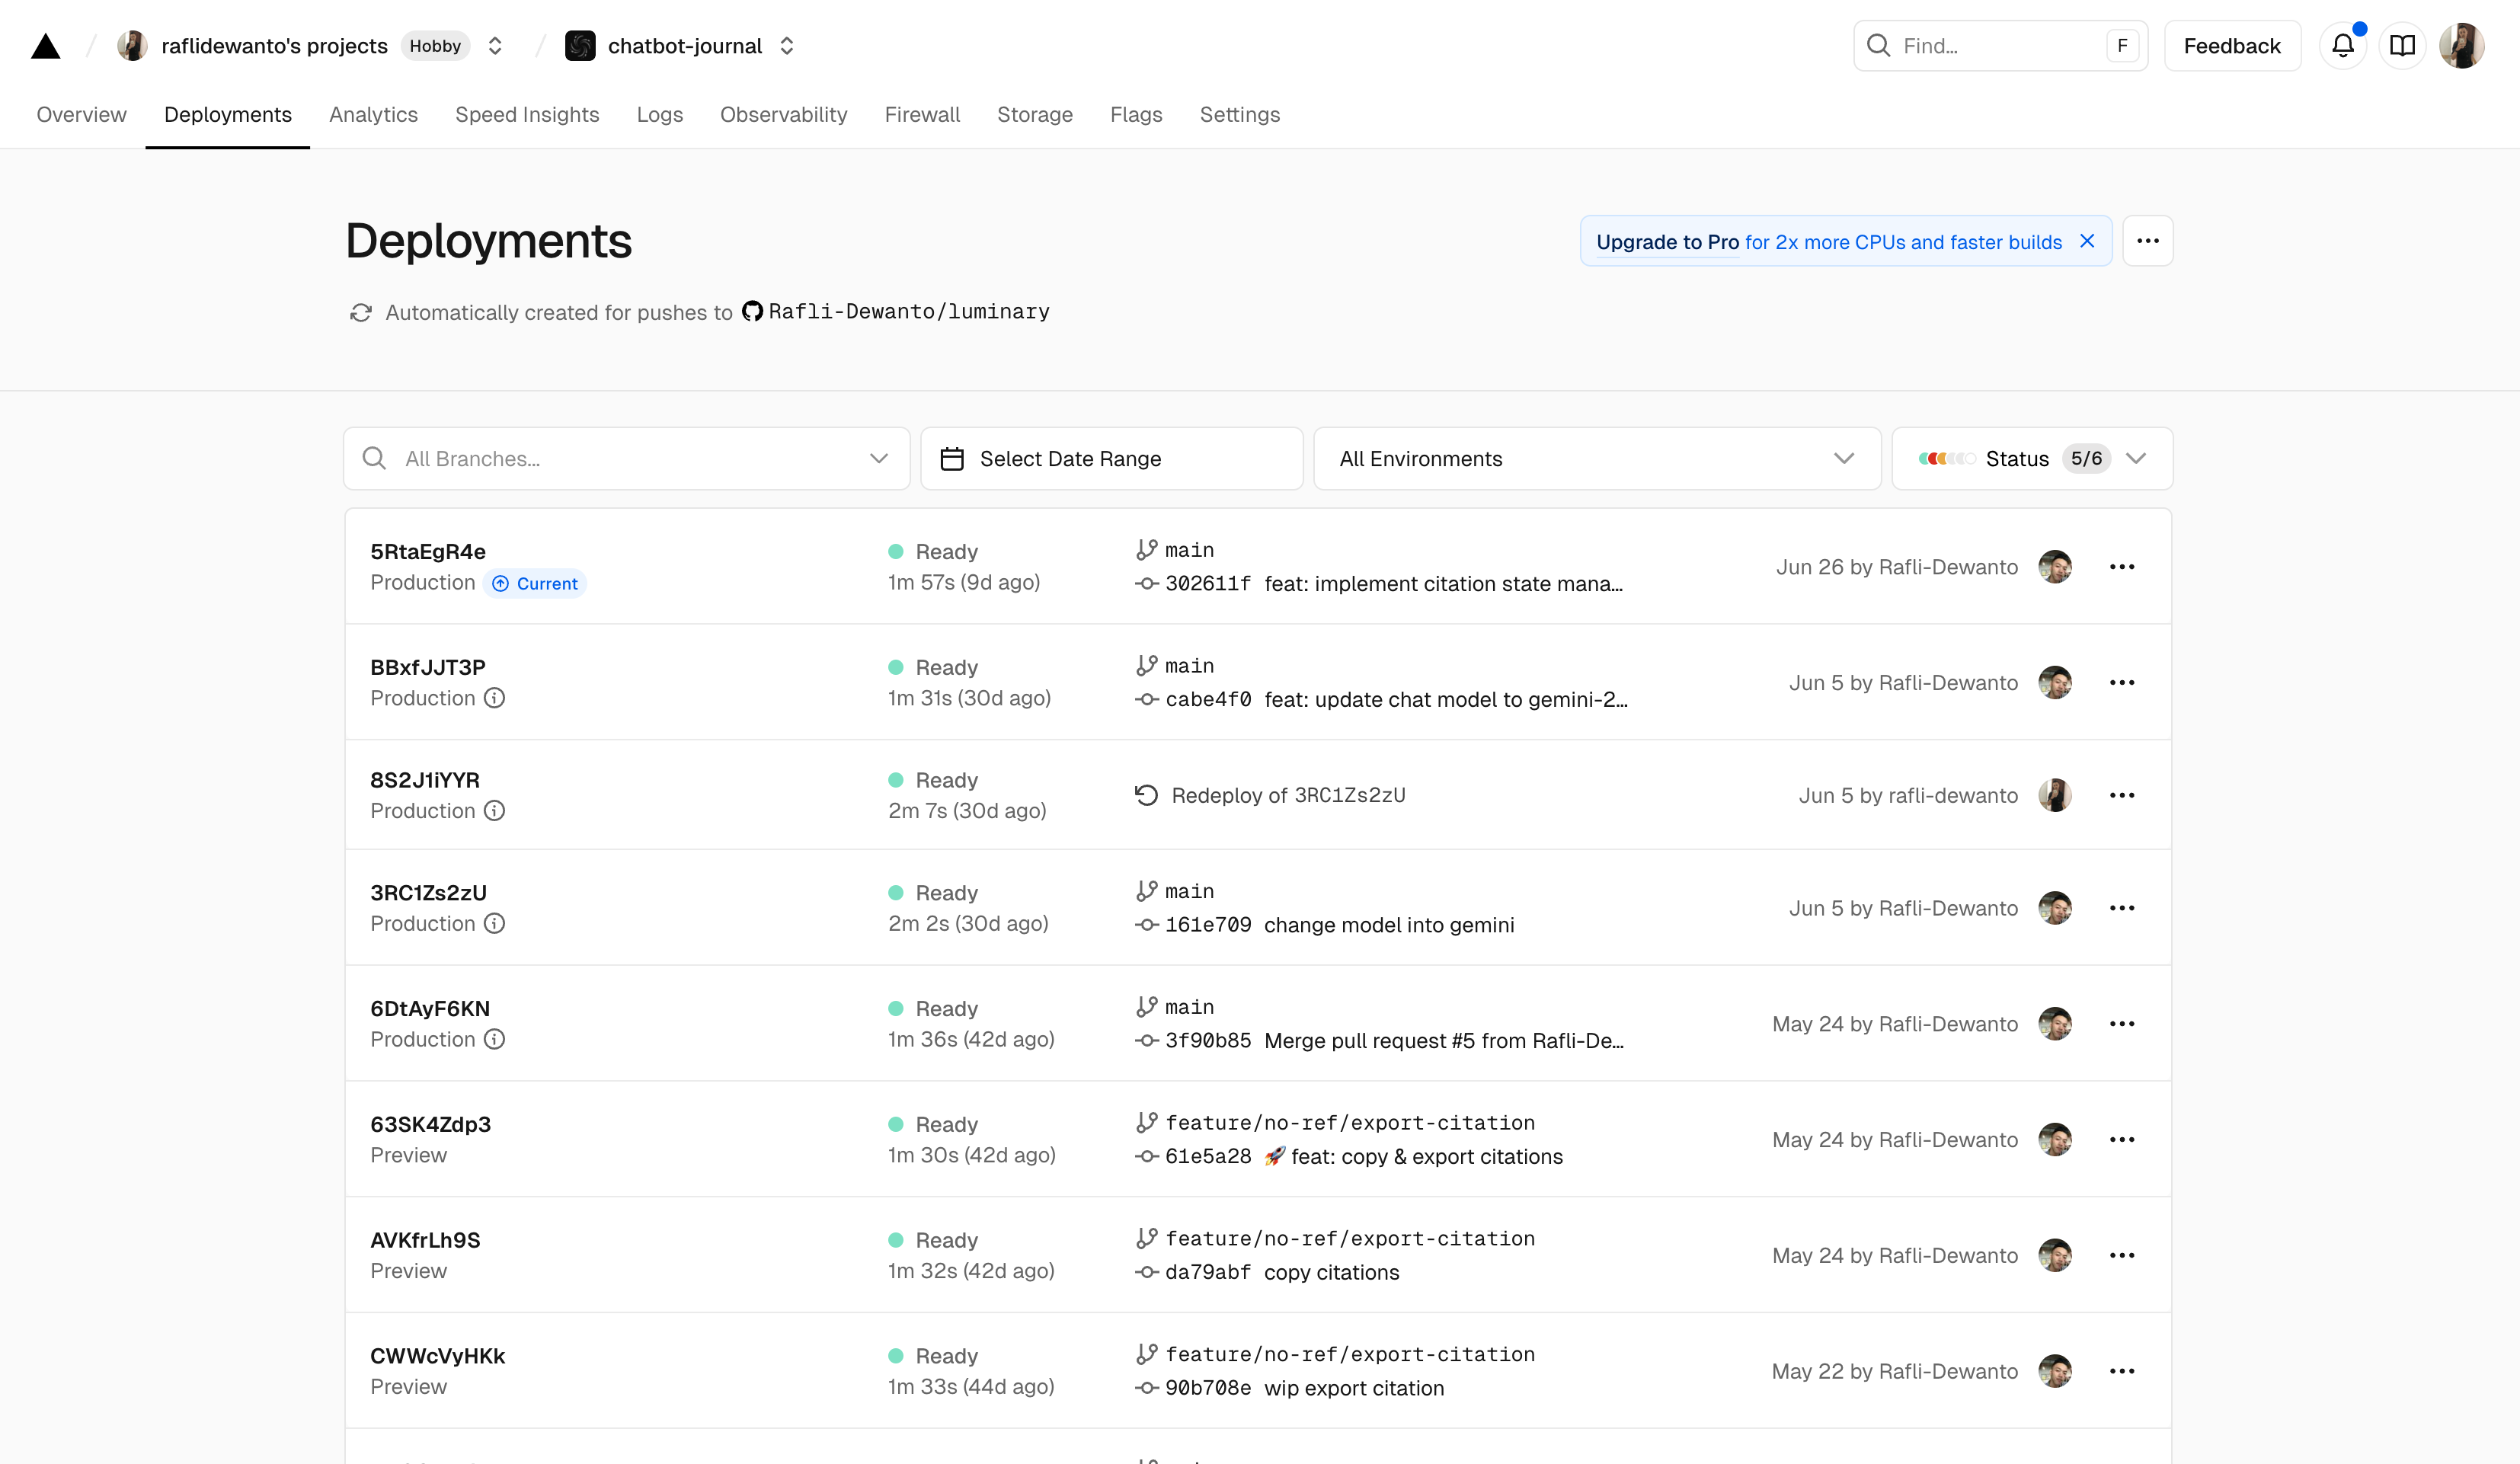
\includegraphics[width=0.85\linewidth]{images/bab-3/deploy-4.png}
  \caption{Aplikasi berhasil dideploy dan tersedia secara publik}\label{fig:finish-deploy}
\end{figure}